\documentclass[12pt, oneside]{book}
\usepackage[a4paper,top=2.5cm,bottom=2.5cm,left=3.5cm,right=2cm]{geometry}
\usepackage[utf8]{inputenc}
\usepackage[T1]{fontenc}
\usepackage{graphicx}
\usepackage{url}
%\usepackage[slovak]{babel} % vypnite pre prace v anglictine
\linespread{1.25} % hodnota 1.25 by mala zodpovedat 1.5 riadkovaniu

% my includes
\usepackage{color}
\usepackage{tocloft}
\usepackage{comment}
\usepackage{moreverb}

% -------------------
% --- Definicia zakladnych pojmov
% --- Vyplnte podla vasho zadania
% -------------------
\def\mfrok{2016}
%\def\mfnazov{Názov vašej bakalárskej práce}
%\def\mftyp{Bakalárska práca}
%\def\mfautor{Meno Priezvisko, príp. tituly}
%\def\mfskolitel{tit. Meno Priezvisko, tit. }
\def\mfnazov{Image-based steganography using a~mobile~phone}
\def\mftyp{Bachelor's thesis}
\def\mfautor{Askar Gafurov}
\def\mfskolitel{RNDr. Michal Forišek, PhD.}

%ak mate konzultanta, odkomentujte aj jeho meno na titulnom liste
\def\mfkonzultant{tit. Meno Priezvisko, tit. }  

\def\mfmiesto{Bratislava, \mfrok}

%aj cislo odboru je povinne a je podla studijneho odboru autora prace
%\def\mfodbor{2508 Informatika} 
%\def\program{ Informatika }
%\def\mfpracovisko{ Katedra informatiky }
\def\mfodbor{2508 Computer Science} 
\def\program{ Computer Science }
\def\mfpracovisko{ Department of Computer Science }

%% my macros
\def\TODO{\textbf{\textcolor{red}{TODO }}}

\begin{document}     

% -------------------
% --- Obalka ------
% -------------------
\thispagestyle{empty}

\begin{center}
\sc\large
%Univerzita Komenského v Bratislave\\
%Fakulta matematiky, fyziky a informatiky
Comenius University in Bratislava\\
Faculty of Mathematics, Physics and Informatics


\vfill

{\LARGE\mfnazov}\\
\mftyp
\end{center}

\vfill

{\sc\large 
\noindent \mfrok\\
\mfautor
}

\eject % EOP i
% --- koniec obalky ----

% -------------------
% --- Titulný list
% -------------------

\thispagestyle{empty}
\noindent

\begin{center}
\sc  
\large
%Univerzita Komenského v Bratislave\\
%Fakulta matematiky, fyziky a informatiky
Comenius University in Bratislava\\
Faculty of Mathematics, Physics and Informatics

\vfill

{\LARGE\mfnazov}\\
\mftyp
\end{center}

\vfill

\noindent
\begin{tabular}{ll}
%Študijný program: & \program \\
%Študijný odbor: & \mfodbor \\
%Školiace pracovisko: & \mfpracovisko \\
%Školiteľ: & \mfskolitel \\
Study program: & \program \\
Branch of studies: & \mfodbor \\
%Školiace pracovisko: & \mfpracovisko \\
Supervisor: & \mfskolitel \\
% Konzultant: & \mfkonzultant \\
\end{tabular}

\vfill


\noindent \mfmiesto\\
\mfautor

\eject % EOP i


% --- Koniec titulnej strany


% -------------------
% --- Zadanie z AIS
% -------------------
% v tlačenej verzii s podpismi zainteresovaných osôb.
% v elektronickej verzii sa zverejňuje zadanie bez podpisov

\newpage 
\thispagestyle{empty}
\hspace{-2cm}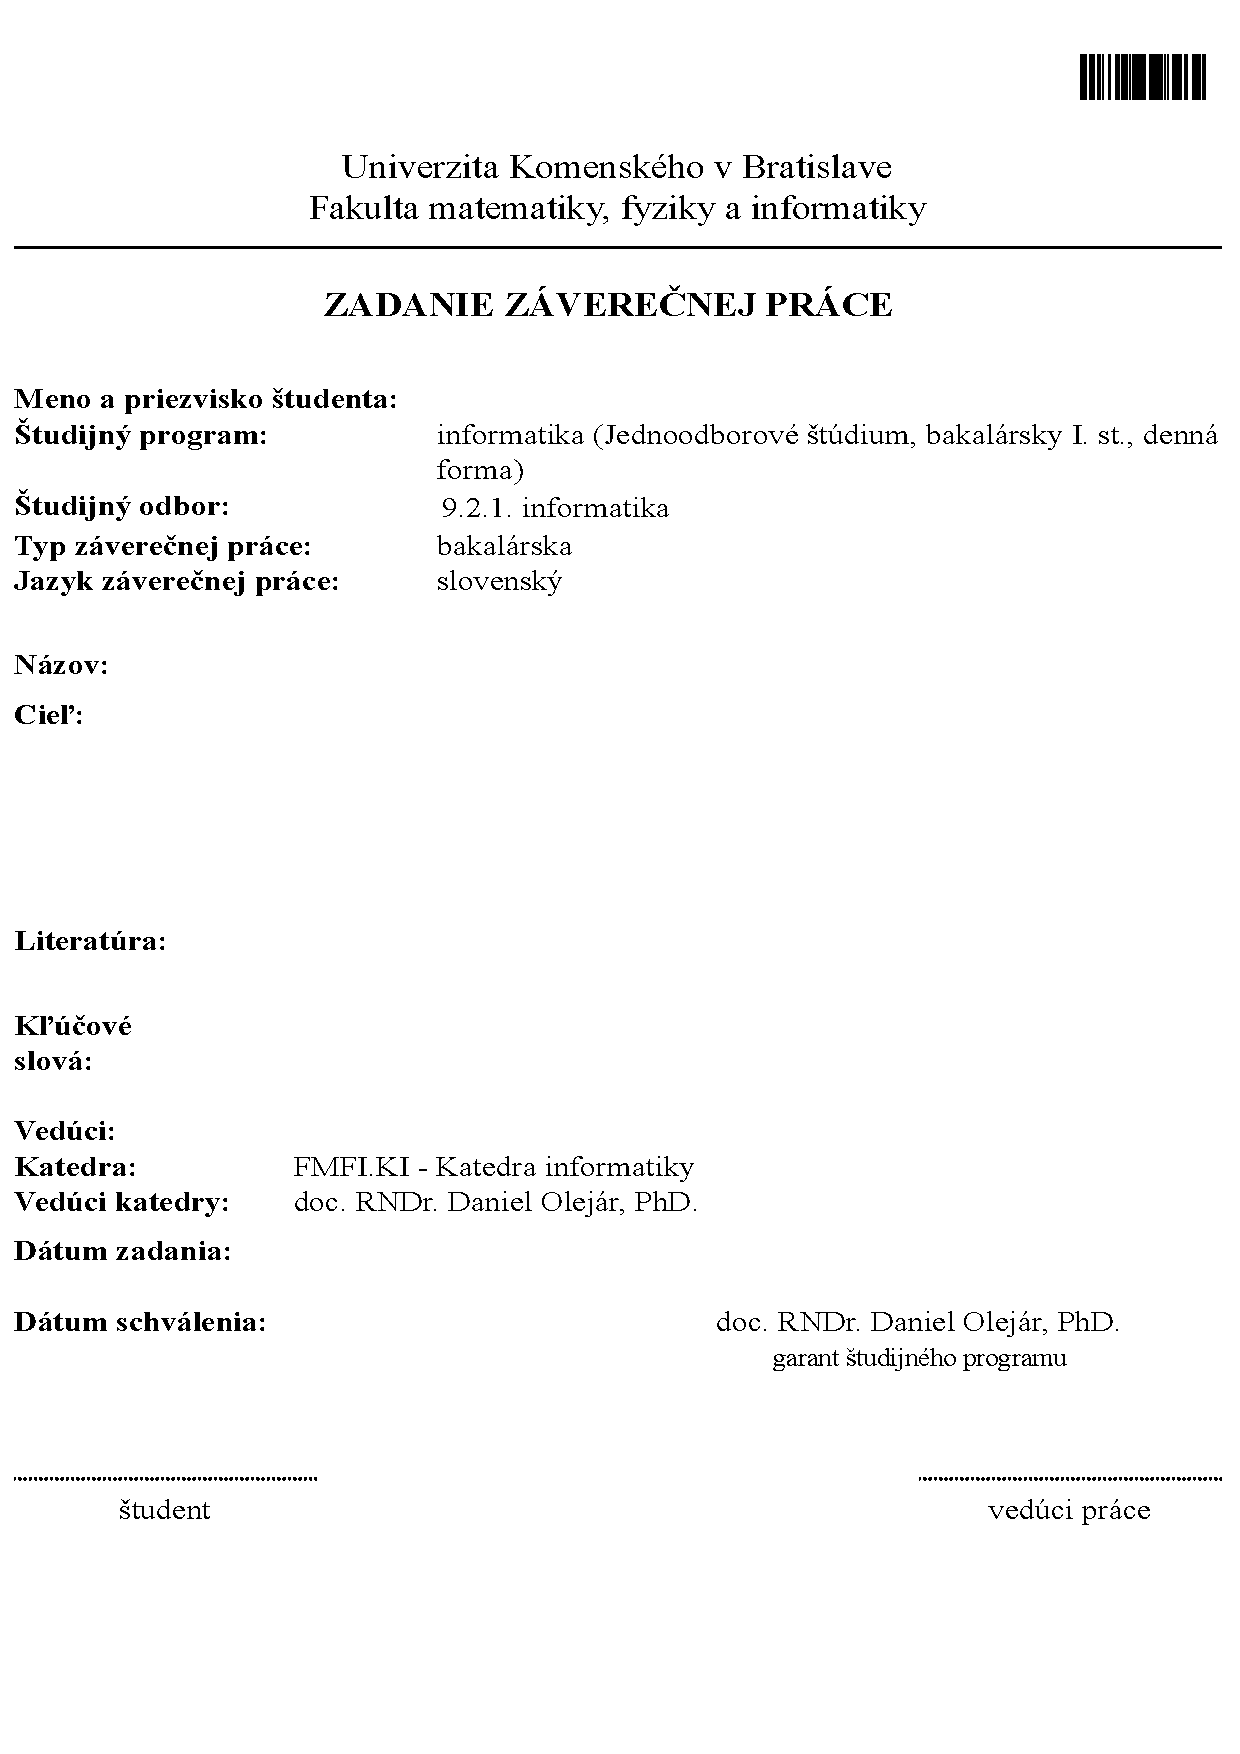
\includegraphics[width=1.1\textwidth]{images/zadanie}

% --- Koniec zadania

\frontmatter

% -------------------
%   Poďakovanie - nepovinné
% -------------------
\setcounter{page}{3}
\newpage 
~

\vfill
%{\bf Poďakovanie:}
{\bf Acknowledgements:}

I'd like to thank my supervisor RNDr. Michal Forišek, PhD. 
for ignoring my e-mails and thus cotributing to my independence
and character development.

\vfill

% --- Koniec poďakovania

% -------------------
%   Abstrakt - Slovensky
% -------------------
\newpage 
\section*{Abstrakt}


Slovenský abstrakt v rozsahu 100-500 slov, jeden odstavec. Abstrakt
stručne sumarizuje výsledky práce. Mal by byť pochopiteľný pre bežného
informatika. Nemal by teda využívať skratky, termíny alebo označenie
zavedené v práci, okrem tých, ktoré sú všeobecne známe.

\TODO Abstrakt v slovencine

\paragraph*{Kľúčové slová:} steganografia, Android, open-source, JPEG, komplementárne vkládanie 
% --- Koniec Abstrakt - Slovensky


% -------------------
% --- Abstrakt - Anglicky 
% -------------------
\newpage 
\section*{Abstract}

\TODO abstract in English

\paragraph*{Keywords:} steganography, Android, open-source, JPEG, complementary embedding

% --- Koniec Abstrakt - Anglicky

% -------------------
% --- Obsah
% -------------------

\newpage 

\tableofcontents

% ---  Koniec Obsahu

% -------------------
% --- Zoznamy tabuliek, obrázkov - nepovinne
% -------------------

\newpage 

\listoffigures

% ---  Koniec Zoznamov

\mainmatter

\input introduction.tex

%\part{EXISTED KNOWLEDGE}

\input steganography.tex

%\part{OUR WORK}

\input goals.tex

\input theory.tex

\input implementation.tex

\input summary.tex

% -------------------
% --- Bibliografia
% -------------------


\newpage	

\backmatter

\thispagestyle{empty}
\nocite{*}
\clearpage

\bibliographystyle{plain}
\bibliography{literatura} 


% -------------------
%--- Prilohy---
% -------------------

%Nepovinná časť prílohy obsahuje materiály, ktoré neboli zaradené priamo  do textu. Každá príloha sa začína na novej strane.
%Zoznam príloh je súčasťou obsahu.
%
%\addcontentsline{toc}{chapter}{Appendix A}
%\input manual.tex
%
%\addcontentsline{toc}{chapter}{Appendix B}
%\input AppendixB.tex

\end{document}
